%Efficient computation
Dado que los problemas financieros son de corriente de datos, es decir, a medida que avanza el tiempo
aparecen nuevos ticks con información para el modelo, no es posible incluir todos estos en un solo modelo.
Por lo tanto se propone una versión online del VECM con la posibilidad de actualizar el modelo con la nueva data y entregar respuestas en un corto perdiodo de tiempo (mínimo menor a la frecuencia).

Obtener los vectores de cointegración usando el método de Johansen es también un procedimiento costoso en cuanto a tiempo computacional. Sin embargo, como los vectores de cointegración representan la relación a largo plazo entre series de tiempo, no varian mucho en el tiempo. El algoritmo propuesto obtiene nuevos vectores de cointegración solamente cuando la relación a largo plazo cambia. Este cambio se detecta siguiendo
en cada paso el cambio del \emph{Mean Absolute Percentage Error} (MAPE) de los últimos n-ajustes del modelo.

Dado que VECM es un modelo basado en las series tiempo diferenciadas, el MAPE es obtenido de $\Delta \mathbf{y}$ de la siguiente forma:

\begin{equation}\label{eq:MAPE}
\text{MAPE}[t] = \frac{1}{n} \sum_{i=1}^{n} \left| 
\frac{\Delta \mathbf{y}_{\text{true}}[t-i]-\Delta
\mathbf{y}_{\text{pred}}[t-i]}{\Delta \mathbf{y}_{\text{true}[t-i]}}
\right| \, , 
\end{equation}

\noindent donde $\Delta \mathbf{y}_{\text{true}}$ es el valor actual de la serie de tiempo
diferenciada $\mathbf{y}$ y $\Delta \mathbf{y}_{\text{pred}}$ es su predicción actual.

Cómo este número presenta un promedio el cual puede ser poco representativa de la muestra se realiza además un estudio de las propiedades estadísticas clásicas.

\section{Algoritmo Propuesto}

Para formular este algoritmo necesitamos definir primeramente las siguientes matrices:

\begin{equation}
\label{eq:notation}
    \mathbf{A}(t) = 
\left[
  \begin{tabular}{c>{$}c<{$}c}
    --- & \mathbf{a}^{\top}_{t-L} & ---\\
    --- & \mathbf{a}^{\top}_{t-L+1} & ---\\
    & \vdots & \\
    --- & \mathbf{a}^{\top}_{t} & ---
  \end{tabular}
\right]
\quad \text{y} \quad
\mathbf{B} =
\left[
  \begin{tabular}{c>{$}c<{$}c}
    --- & \mathbf{b}_{t-L} & ---\\
    --- & \mathbf{b}_{t-L+1} & ---\\
    & \vdots & \\
    --- & \mathbf{b}_{t} & ---
  \end{tabular}
\right] \, ,
\
\end{equation}

La solución optima usando ventanas deslizantes es:

\begin{eqnarray}
\label{eq:optsolSLAAR}
\mathbf{X}(t)&=&({\bf A}(t)^\top{\bf A}(t)+
\gamma \mathbb{I})^{-1}{\bf A}(t)^\top{\bf B}(t) \\
\mathbf{X}(t)&=&\mathbf{S}(t)^{-1} \mathbf{W}(t) \, ,
\end{eqnarray}



\subsection{Diagrama de Clases}
La implementación fue realizada en Python, usando principalmente las bibliotecas:
\begin{itemize}
 \item Pandas: biblioteca para manipulación y análisis de datos. \footnote{\url{http://pandas.pydata.org}}
 \item Statsmodels: módulo que permite explorar data, estimar modelos y test
estadísticos. \footnote{\url{}}
 \item Numpy: paquete de computación científica en Python, provee estructuras
de datos y funciones de álgebra lineal entre otras cosas.
\footnote{\url{http://www.numpy.org}}
 \item Scikit.CUDA: provee interfaces a un set de funciones de CUDA, cuBLAS y
otras bibliotecas. La idea es poder ejecutar funciones de cuda desde python a
través de wrappers. \footnote{\url{http://scikits.appspot.com/cuda}}
\end{itemize}

Basándose en esas bibliotecas y otras más, se crearon 3 clases mostrados en la
figura \ref{fig:class_diagram}:
\begin{itemize}
 \item Util: provee métodos generales utilizados por las otras 2 clases.
 \item Reader: clase que lee los datos ticks desde archivos CSV descargados
desde dukascopy, provee funciones para juntar monedas en la misma estructura de
datos, hacer resampling a cierta frecuencia y normalizar monedas, entre otras
funciones.
 \item Matrix: es la clase es más extensa y contiene los principales métodos
utilizados por los algoritmos, entre ellos la creación de las matrices VAR y
VECM, el update de las matrices optimizado para la ventana deslizante, cálculo
de vectores de integración mediante Johansen, test de estacionaridad usando
Augmented Dicky Fuller, Errores porcentuales, etc.
\end{itemize}

\begin{figure}[h!t]
    \begin{center}
        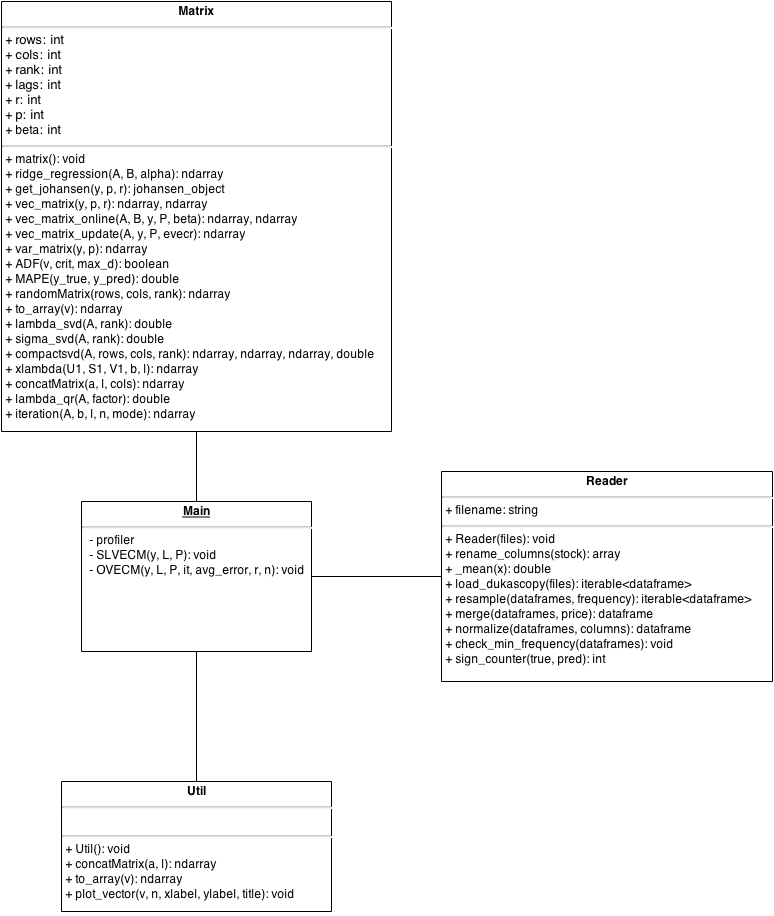
\includegraphics[width=0.8\textwidth]{images/class_diagram.png}
        \caption{Diagrama de Clases}
        \label{fig:class_diagram}
    \end{center}
\end{figure}

\section{Métodos a paralelizar}
